\documentclass{article}
\usepackage[final]{nips_2017}
\usepackage[utf8]{inputenc} % allow utf-8 input
\usepackage[T1]{fontenc}    % use 8-bit T1 fonts
\usepackage{hyperref}       % hyperlinks
\usepackage{url}            % simple URL typesetting
\usepackage{booktabs}       % professional-quality tables
\usepackage{amsfonts}       % blackboard math symbols
\usepackage{nicefrac}       % compact symbols for 1/2, etc.
\usepackage{microtype}      % microtypography
\usepackage{graphicx}
\usepackage{amsmath}
\usepackage{tikz}
\usetikzlibrary{positioning, shapes.geometric, arrows.meta}
\usepackage{natbib}
\bibliographystyle{unsrtnat}
\usepackage{hyperref}
\usepackage{float}
\usepackage{xcolor}
\usepackage{tcolorbox}
\usepackage{xcolor,soul}
\sethlcolor{cyan!30} % Sets light blue as highlight color

\newcommand{\hlblue}[1]{\hl{#1}}

\title{Automated LaTeX Code Generation from Handwritten Mathematical Expressions \\
Category: Computer Vision}

\author{
  Jayaprakash Sundararaj \\
  \texttt{osjp@stanford.edu}  \\
  \AND
  Akhil Vyas \\
  \texttt{avyas21@stanford.edu}  \\
  \AND
  Benjamin Gonzalez-Maldonado \\
  \texttt{bengm@stanford.edu } \\
}

\begin{document}
% \nipsfinalcopy is no longer used

\begin{center}

\includegraphics[width=3cm, height=0.7cm]{CS230}
\end{center}

\maketitle

\begin{abstract}
Converting mathematical expressions into LaTeX is challenging. In this paper, we explore using newer transformer based architectures for addressing the problem of converting handwritten/digital mathematical expression images into equivalent LaTeX code. We use the current state of the art CNN encoder and RNN decoder as a baseline for our experiments. We also investigate improvements to CNN-RNN architecture by replacing the CNN encoder with the ResNet50 model. Our experiments show that transformer architectures achive a \~2.7\% higher overall accuracy compared to the CNN/RNN architectures with room to achieve even better results with appropriate fine-tuning of model parameters.
\end{abstract}

\section{Introduction}	

Converting handwritten mathematical expressions into digital formats is time consuming, specifically LaTeX code. Our goal is to train a ML model that is capable of encoding handwritten notes and converting to the source code seamlessly. The input to our algorithm is an image of a handwritten mathematical expression. The challenge of our project is to convert an image to a text LaTeX sequence which will require the use of both computer vision and NLP techniques. 

% Explain the problem and why it is important. Discuss your motivation for pursuing this
% problem. Give some background if necessary. Clearly state what the input and output
% is. Be very explicit: “The input to our algorithm is an {image, amplitude, patient age,
% rainfall measurements, grayscale video, etc.}. We then use a {SVM, neural network, linear
% regression, etc.} to output a predicted {age, stock price, cancer type, music genre, etc.}.”
% This is very important since different teams have different inputs/outputs spanning different
% application domains. Being explicit about this makes it easier for readers. If you are using
% your project for multiple classes, add a paragraph explaining which components of the
% project were used for each class.

\section{Related work}
% [You should find existing papers, group them into categories based on their approaches,
% and discuss their strengths and weaknesses, as well as how they are similar to and differ
% from your work. In your opinion, which approaches were clever/good? What is the stateof-the-art?
% Do most people perform the task by hand? You should aim to have at least
% 5 references in the related work. Include previous attempts by others at your problem,
% previous technical methods, or previous learning algorithms. Google Scholar is very useful
% for this: https://scholar.google.com/ (you can click “cite” and it generates MLA, APA,
% BibTeX, etc.)]
\cite{schechter2017converting} investigated a variety of methods like neural networks, CNNs, Random Forests, SVMs, OCR, CGrp, and SA. However, most state of the art  methods utilize encoder-decoder architectures involving CNNs and LSTM architectures like \cite{genthial2016image}. In recent works like \cite{bian2022handwritten}, both left-to-right and right-to-left decoders are utilized. The CNN-RNN architecture will serve as a baseline for our work.

Transformer architectures (\cite{transformer}) are currently achieving the best results for NLP tasks . \cite{visiontransformer} introduced vision transformers which uses sequences of image patches to replace convolutions. We will leverage a vision transformer encoder and transformer decoder architecture and compare it to the baseline.

\section{Dataset and Features}

We will use the datasets from two main repositories: \texttt{Im2latex-100k} (\cite{kanervisto_2016_56198}) and \texttt{Im2latex-230k} (\cite{gervais2024mathwritingdatasethandwrittenmathematical}). The \texttt{Im2latex-100k} (\cite{kanervisto_2016_56198}) dataset, available at \href{https://zenodo.org/records/11230382}{Zenodo}, contains 100,000 image-formula pairs. The \texttt{Im2latex-230k} (\cite{gervais2024mathwritingdatasethandwrittenmathematical}) 
 dataset, also known as \texttt{Im2latexv2}, contains 230,000 samples. It includes both OpenAI-generated and handwritten examples, further enhancing the diversity of the data. This dataset is available at \href{https://im2markup.yuntiandeng.com/data/}{Im2markup}. The training data format is \texttt{<image file name> <formula id>}.
 
 The dataset disk size is 849 MB. The images are gray scales with 50x200 pixels. The numbers of symbols (\autoref{fig:formula_length}) in the latex formulas vary from range varies from 1 to 150 symbols. Voabulary contains 540 symbols, refer \autoref{fig:vocab_freq_1} and \autoref{fig:vocab_freq_2} for the list of popular and least occurring symbols with their frequency.
 
\begin{figure}[H]
    \centering
    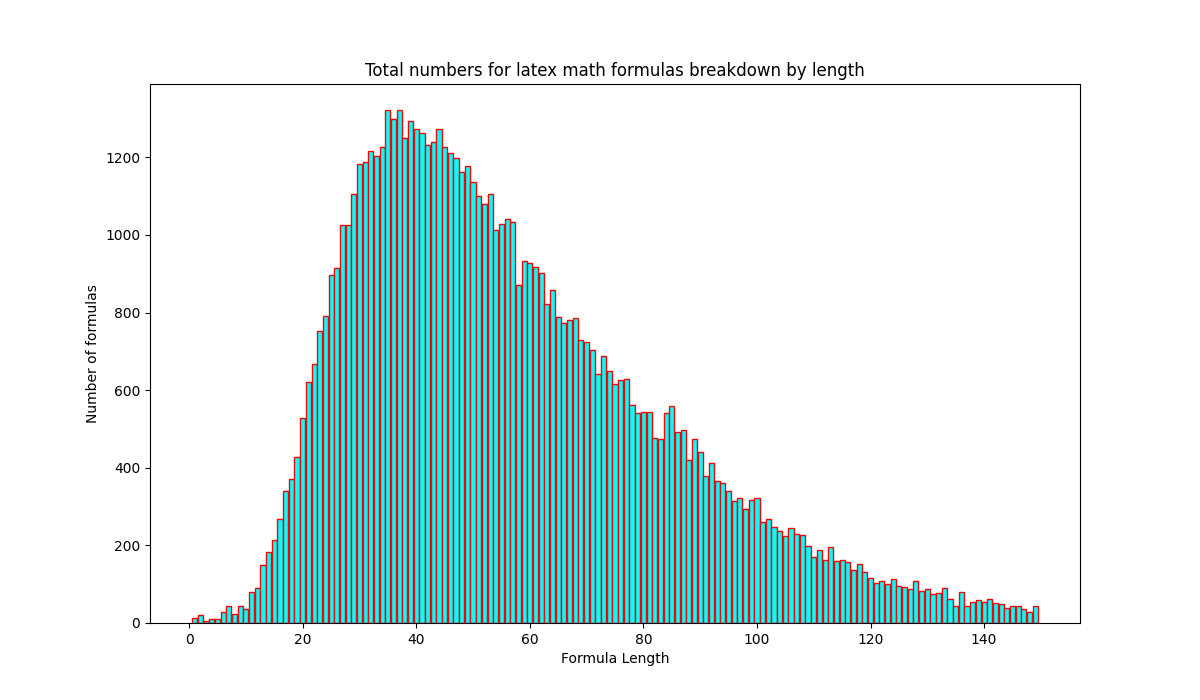
\includegraphics[scale=0.4]{fig_latex_formula_length.png}
    \caption{Formulas breakdown by length}
    \label{fig:formula_length}
\end{figure}

\section{Methods}

\subsection{CNN encoder and GRU/LSTM}
As a baseline, We use the CNN Encoder to encode the image input of resized image (50x200) with 1 channel (greyscale). We use 3x3 convolutional filter followed by 2x2 max pooling layer. This previous block is repeated three times and followed fully connected layer.

\begin{figure}[H]
    \centering
    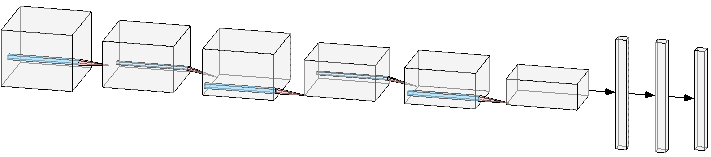
\includegraphics[scale=0.6]{cnn_architecture.png}
    \caption{Encoder architecture consists of 3 convolution-max pooling blocks (50,200) -> (25,100) -> (12,5) which is flattened and fed into Dense layer (256 units)  }	
    \label{fig:cnn_lstm}
\end{figure}

During decoding, We compute the embedding for formula tokens and concatenated with image encoded embedding. The concatenation of image and token embedding fed into LSTM/GRU units, followed by fully connected network. The activation is softmax.  Overall model architecture is: 
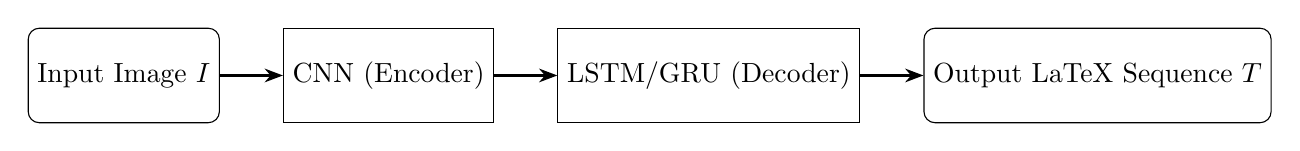
\begin{tikzpicture}[
    node distance=1cm, 
    every node/.style={rectangle, draw, minimum height=1.2cm, minimum width=1cm, align=center},
    arrow/.style={-Stealth, thick}
]

% Nodes
\node (input) [rounded corners] {Input Image \(I\)};
\node (cnn) [right=0.8cm of input] {CNN (Encoder)};
\node (lstm) [right=0.8cm of cnn] {LSTM/GRU (Decoder)};
\node (output) [right=0.8cm of lstm, rounded corners] {Output LaTeX Sequence \(T\)};

% Arrows
\draw [arrow] (input) -- (cnn);
\draw [arrow] (cnn) -- (lstm);
\draw [arrow] (lstm) -- (output);

\end{tikzpicture}

\subsection{LSTM with funetuning with pretrained Resnet50}

Here we use the pretained ResNet50 model as a encoder (98Mb disk size). However, ResNet50 expects the image with fixed size 254x254 and 3 channels. Our input images are grey scale. So, we transform the input image to the ResNet50 input using \verb|tf.keras.layers.Lambda(lambda x: tf.image.grayscale_to_rgb(x)|.


\begin{figure}[H]
    \centering
    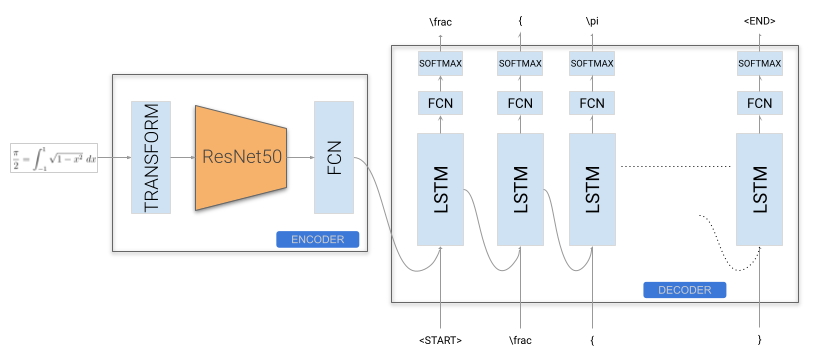
\includegraphics[scale=0.42]{fig_resnet_LSTM.png}
    \caption{Pretrained ResNet50 Encoder with LSTM Decoder.}
    \label{fig:resnet_lstm}
\end{figure}

\subsection{Vision transformer encoder and transformer decoder}

\subsubsection{Vision Transformer Encoder}
The vision encoder leverages patches of the image. We create patches of 10 X 10. Since our images are of size 50 X 200, we have a total of 100 patches per image.
\begin{figure}[h]
	\centering 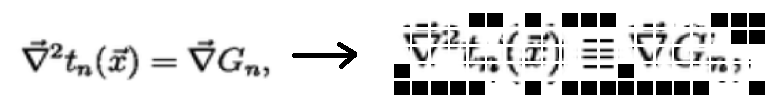
\includegraphics[scale=0.5]{image_to_patches.png}
	\caption{Original latex image and the generated patches}
\end{figure}

In the vision transformer encoder, these patches are taken and embedded linearly and added to the positional embeddings. That is fed into a standard transformer layer. We use 8 transformer layers for our architecture that have 4 attention heads and 2 layer multi-layer perceptron with 2048 and 1024 units.

\begin{figure}[H]
	\centering 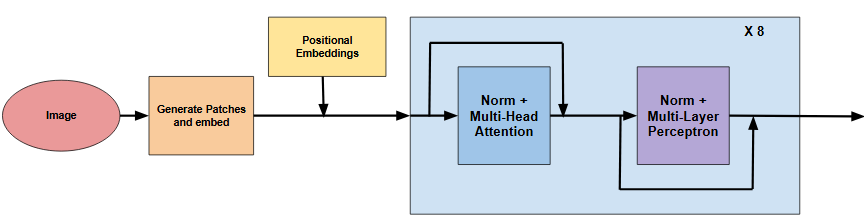
\includegraphics[scale=0.75]{transformer_encoder.png}
	\caption{Transformer encoder architecture}
\end{figure}

\subsubsection{Vision Transformer Decoder}

We use the standard transformer block for the decoder which uses cross-attention to find parts of the image to focus on and self-attention for the sequence generation. Our configuration uses 4 attention layers with 8 heads for both the self-attention and cross-attention components in each layer.

\begin{figure}[H]
	\centering 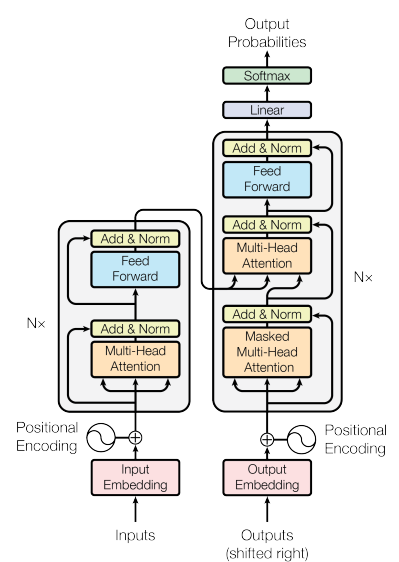
\includegraphics[scale=0.7]{transformer_decoder.png}
	\caption{Transformer encoder architecture from \cite{transformer}}
\end{figure}


\section{Experiments}

\subsection{Setup/Metrics}

We use a single AWS G6.xlarge instance to train the models on 50,000 data points. The training time varies between  1 hr 30 mins and 2 hrs. We use early stopping with a patience of 10. We compute the following metrics to compare the baseline and other methods:

\begin{itemize}
  \item We measure the `sparse categorical loss` and accuracy which measures the loss/accuracy accross all tokens. 
  \item We measure the masked loss and accuracy to measure the accuracy for the non-padded tokens (we pad our tokens to length 151 and this will only check the loss/accuracy for the tokens that are part of the label sequence)
\end{itemize}

\subsection{CNN-RNN baseline}
We explored using both LSTM/GRU for the decoder and the difference between the two were negligible. Here are the training curves with  CNN - LSTM/GRU architectures:
\newline \newline
 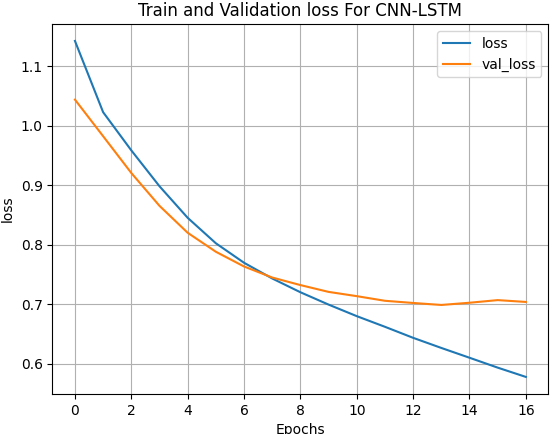
\includegraphics[scale=0.45]{lstm_training.png}
 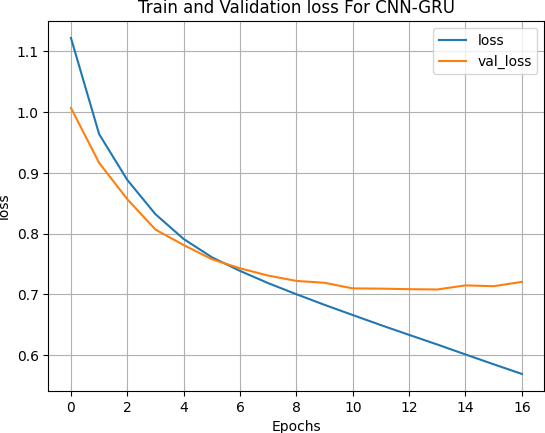
\includegraphics[scale=0.45]{gru_training.png}

Both models had ~85\% accuracy with GRU being slightly worse off. Due to this, we used the numbers from the LSTM decoder to compare against the other models. 

\subsection{Results}
\begin{center}
\begin{tabular}{||c | c | c | c | c||} 
 \hline
 Architecture & Loss & Accuracy & Masked Loss & Masked Accuracy \\ [0.5ex] 
 \hline\hline
 CNN-RNN (LSTM) & 0.6479 & 0.8470 & 1.6941 & 0.6008 \\ 
 \hline
 Vision Transformer Encoder + Transformer Decoder  & 0.5209 & 0.8738 & 1.4722 & 0.6417 \\
 \hline
\end{tabular}
\end{center}

We can see that the transformer architecture gets significantly lower loss and higher accuracy compared to the baseline CNN-RNN model.

\section{Conclusion/Future Work}
We can see that the transformer architecture outperformed the vanilla CNN-RNN architecture on all measured metrics. Given more time, we would have mainly focused on experimenting with various transformer architecture configurations (by changing number of layers, attention heads, patch size for the vision transformer encoder etc.)

\section{Contributions}

\textbf{Jayaprakash Sundararaj}: Initial report, researching the dataset and existing methods. Implementing the full CNN and LSTM as a baseline. Extending to pre-trained ResNet50 model with finetuning.

\textbf{Akhil}: Ideation, AWS/GPU setup, Extending to CNN + GRU as a baseline, vision transformer encoder + transformer decoder model, masked loss and accuracy.

\textbf{Ben}: \hlblue{TODO}

\medskip

\nocite{*}
\bibliography{sample}

\section{Appendix}

\begin{figure}[H]
    \centering
    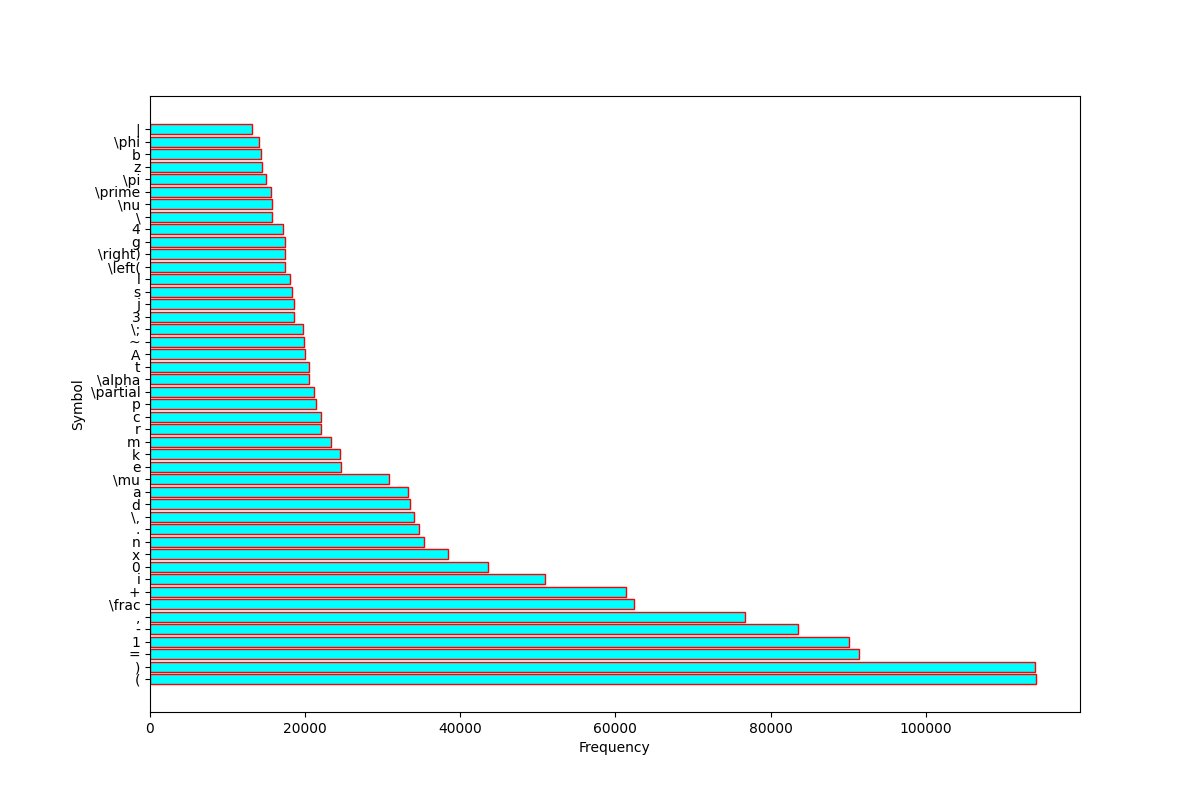
\includegraphics[scale=0.4]{fig_vocabs_frequency_1.png}
    \caption{Dataset: Most popular symbols and frequencies.}
    \label{fig:vocab_freq_1}
\end{figure}

\begin{figure}[H]
    \centering
    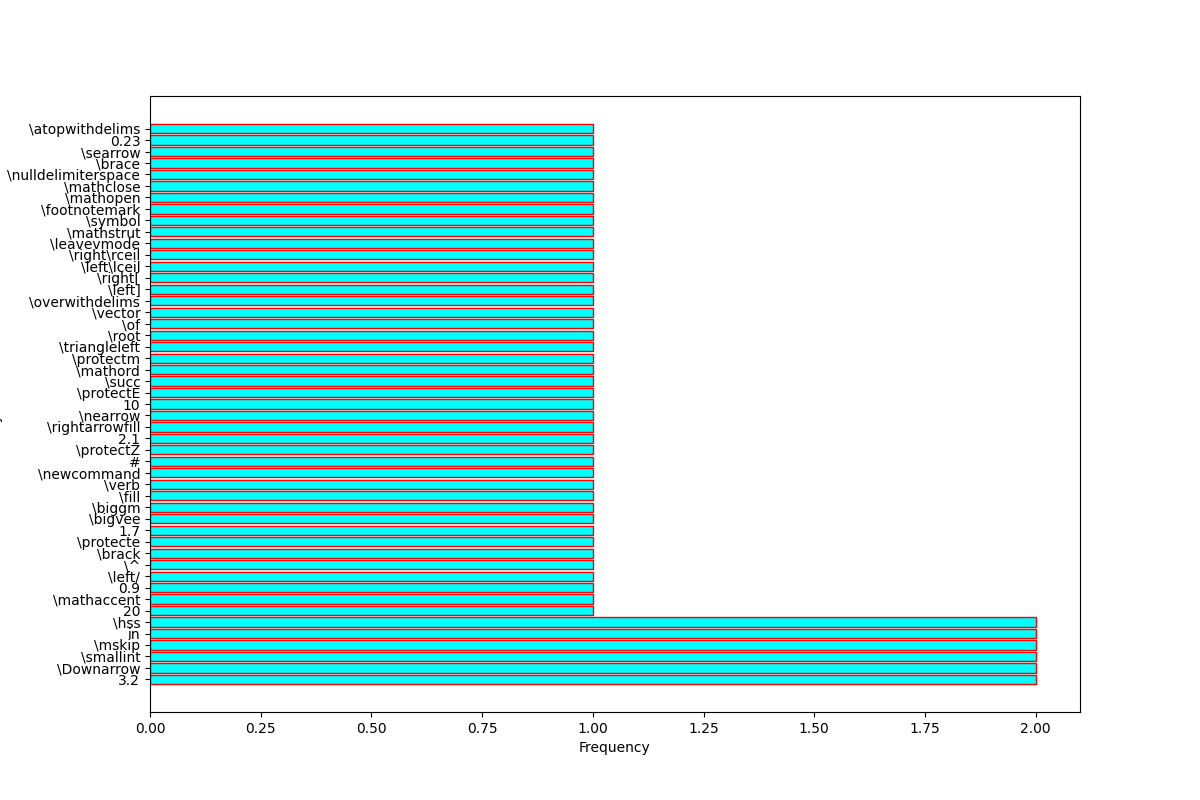
\includegraphics[scale=0.4]{fig_vocabs_frequency_2.png}
    \caption{Dataset: Least popular symbols and frequencies.}
    \label{fig:vocab_freq_2}
\end{figure}


\end{document}